% readme-figures.tex -- the two plans as images for the README:
%   lualatex readme-figures.tex
%   pdftocairo -svg -f 1 -l 1 readme-figures.pdf fig-small.svg
%   pdftocairo -svg -f 2 -l 2 readme-figures.pdf fig-large.svg
% (white background, so that the figures stay readable in dark mode)
\documentclass[tikz,border=6pt]{standalone}
\usepackage{fontspec}
\usepackage{unicode-math}
\setmainfont{Libertinus Serif}
\setsansfont{Libertinus Sans}
\setmathfont{Libertinus Math}
\usepackage{xcolor}
\usetikzlibrary{arrows.meta,fit,backgrounds,calc}
\definecolor{cm}{HTML}{6B6B6B}
\definecolor{xfer}{HTML}{D9730D}
\newcommand{\inv}{^{-1}}
\newcommand{\invT}{^{-\mathsf{T}}}
% placement-styles.tex -- TikZ styles of the swimlane figures (needs the
% colours cm and xfer, and the tikz libraries arrows.meta and fit).
\tikzset{
  lane/.style={fill=black!3, draw=none},
  lanelabel/.style={font=\sffamily\small\bfseries, anchor=west},
  op/.style={draw, rounded corners=2pt, fill=blue!6, font=\sffamily\footnotesize,
    align=center, inner sep=2.5pt, minimum height=6mm},
  mat/.style={draw, fill=black!8, font=\footnotesize, inner sep=2.5pt,
    minimum height=5mm},
  io/.style={draw, rounded corners=2pt, fill=green!8, font=\sffamily\footnotesize,
    inner sep=2.5pt, minimum height=6mm},
  t/.style={font=\sffamily\scriptsize, text=cm},
  local/.style={-{Stealth[length=1.8mm]}},
  move/.style={-{Stealth[length=2.2mm]}, very thick, xfer},
  mv/.style={font=\sffamily\scriptsize, text=xfer!80!black, fill=white,
    inner sep=1pt},
  loopbox/.style={draw=cm, dashed, rounded corners=4pt},
}
% \lanes{width}: the four device lanes, CPU on top
\newcommand{\lanes}[1]{%
  \foreach \name/\y in {CPU/0, GPU/-1.5, NPU/-3, FPGA/-4.5} {
    \fill[lane] (0,\y-0.6) rectangle (#1,\y+0.6);
    \node[lanelabel] at (0.1,\y) {\name};
  }}


\tikzset{every picture/.append style={show background rectangle,
  background rectangle/.style={fill=white, draw=none}}}
\begin{document}
% fig-small.tex -- the small-camera plan (see placement.tex)
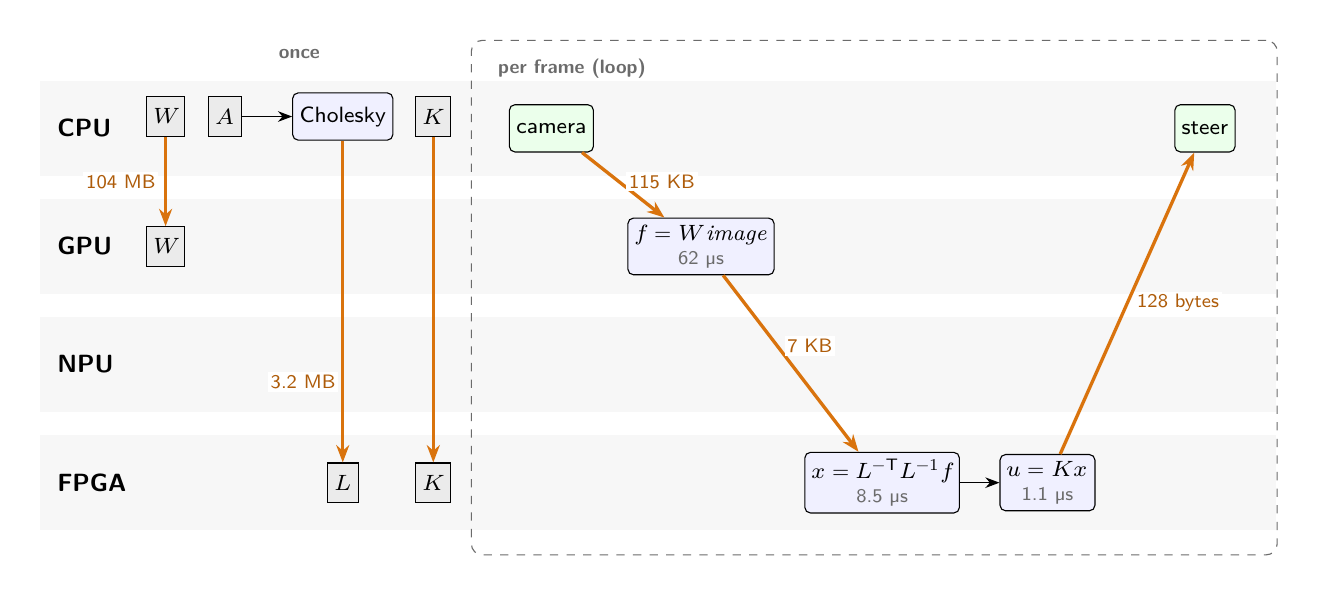
\begin{tikzpicture}[x=1cm,y=1cm]
  \lanes{15.7}
  % once
  \node[font=\sffamily\scriptsize\bfseries, text=cm] at (3.3,0.95) {once};
  \node[mat] (W) at (1.6,0.15) {\(W\)};
  \node[mat] (A) at (2.35,0.15) {\(A\)};
  \node[op] (potrf) at (3.85,0.15) {Cholesky};
  \node[mat] (K) at (5.0,0.15) {\(K\)};
  \node[mat] (Wg) at (1.6,-1.5) {\(W\)};
  \node[mat] (Lf) at (3.85,-4.5) {\(L\)};
  \node[mat] (Kf) at (5.0,-4.5) {\(K\)};
  \draw[local] (A) -- (potrf);
  \draw[move] (W) -- node[mv,left=2pt] {104 MB} (Wg);
  \draw[move] (potrf) -- node[mv,pos=.75,left=1pt] {3.2 MB} (Lf);
  \draw[move] (K) -- (Kf);
  % per frame
  \node[io] (cam) at (6.5,0) {camera};
  \node[op] (gemv) at (8.4,-1.5) {\(f = W\,\mathit{image}\)\\[-1pt]\textcolor{cm}{\scriptsize 62 µs}};
  \node[op] (trsv) at (10.7,-4.5) {\(x = L\invT L\inv f\)\\[-1pt]\textcolor{cm}{\scriptsize 8.5 µs}};
  \node[op] (ctl) at (12.8,-4.5) {\(u = Kx\)\\[-1pt]\textcolor{cm}{\scriptsize 1.1 µs}};
  \node[io] (steer) at (14.8,0) {steer};
  \draw[move] (cam) -- node[mv,pos=.45,right=2pt] {115 KB} (gemv);
  \draw[move] (gemv) -- node[mv,pos=.4,right=2pt] {7 KB} (trsv);
  \draw[local] (trsv) -- (ctl);
  \draw[move] (ctl) -- node[mv,pos=.5,right=2pt] {128 bytes} (steer);
  \node[loopbox, fit={(5.6,1.0) (15.6,-5.3)}] (loop) {};
  \node[font=\sffamily\scriptsize\bfseries, text=cm, anchor=north west] at (5.7,1.0) {per frame (loop)};
\end{tikzpicture}

% fig-large.tex -- the large-camera plan (see placement.tex)
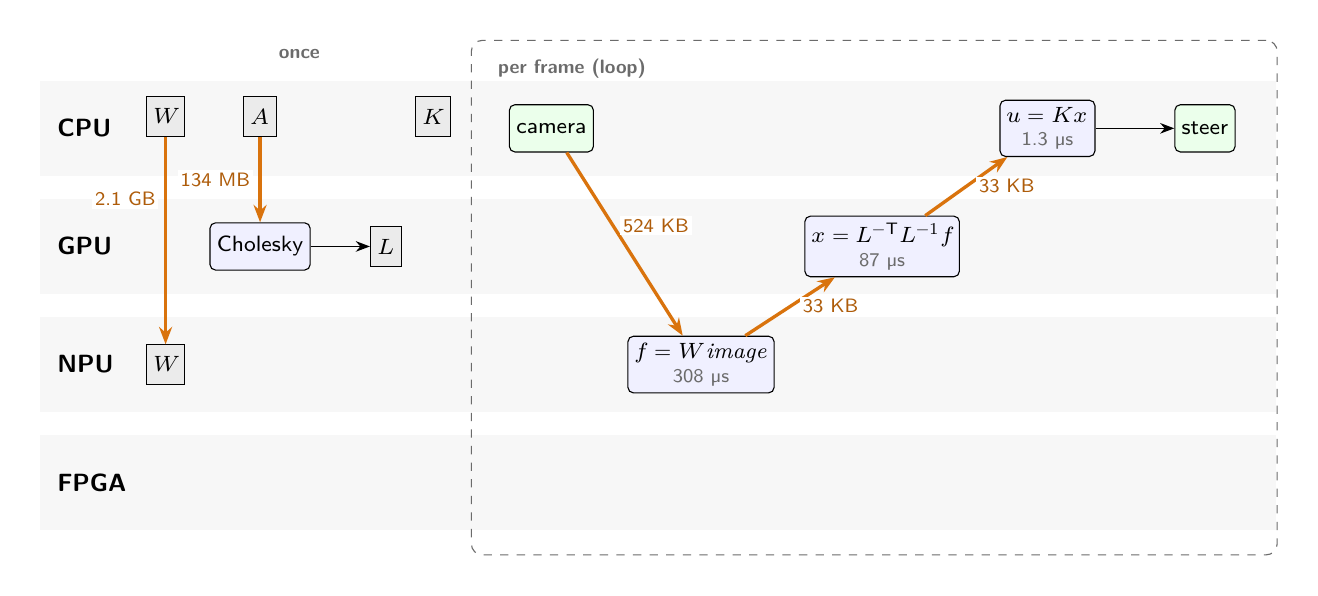
\begin{tikzpicture}[x=1cm,y=1cm]
  \lanes{15.7}
  % once
  \node[font=\sffamily\scriptsize\bfseries, text=cm] at (3.3,0.95) {once};
  \node[mat] (W) at (1.6,0.15) {\(W\)};
  \node[mat] (A) at (2.8,0.15) {\(A\)};
  \node[mat] (K) at (5.0,0.15) {\(K\)};
  \node[op] (potrf) at (2.8,-1.5) {Cholesky};
  \node[mat] (Lg) at (4.4,-1.5) {\(L\)};
  \node[mat] (Wn) at (1.6,-3) {\(W\)};
  \draw[move] (W) -- node[mv,pos=.3,left=2pt] {2.1 GB} (Wn);
  \draw[move] (A) -- node[mv,left=2pt] {134 MB} (potrf);
  \draw[local] (potrf) -- (Lg);
  % per frame
  \node[io] (cam) at (6.5,0) {camera};
  \node[op] (gemv) at (8.4,-3) {\(f = W\,\mathit{image}\)\\[-1pt]\textcolor{cm}{\scriptsize 308 µs}};
  \node[op] (trsv) at (10.7,-1.5) {\(x = L\invT L\inv f\)\\[-1pt]\textcolor{cm}{\scriptsize 87 µs}};
  \node[op] (ctl) at (12.8,0) {\(u = Kx\)\\[-1pt]\textcolor{cm}{\scriptsize 1.3 µs}};
  \node[io] (steer) at (14.8,0) {steer};
  \draw[move] (cam) -- node[mv,pos=.4,right=2pt] {524 KB} (gemv);
  \draw[move] (gemv) -- node[mv,pos=.5,right=3pt] {33 KB} (trsv);
  \draw[move] (trsv) -- node[mv,pos=.5,right=3pt] {33 KB} (ctl);
  \draw[local] (ctl) -- (steer);
  \node[loopbox, fit={(5.6,1.0) (15.6,-5.3)}] (loop) {};
  \node[font=\sffamily\scriptsize\bfseries, text=cm, anchor=north west] at (5.7,1.0) {per frame (loop)};
\end{tikzpicture}

\end{document}
